\part{Data types}
\frame{\partpage}

\begin{frame}{What is a type?}
	\begin{itemize}
		\pause\item A \textbf{variable} in Python holds a \textbf{value}
		\pause\item Every value has a \textbf{type}
		\pause\item The type of a value dictates:
			\begin{itemize}
				\pause\item What sort of data it can hold
				\pause\item How the data is stored in memory
				\pause\item What operations can be done on it
			\end{itemize}
		\pause\item Python is \textbf{weakly typed} --- a variable can hold a value of any type
		\pause\item Many languages are \textbf{strongly typed} --- a variable has a defined type and can only hold values of that type
	\end{itemize}
\end{frame}

\begin{frame}{Memory}
	\pause
	\begin{center}
		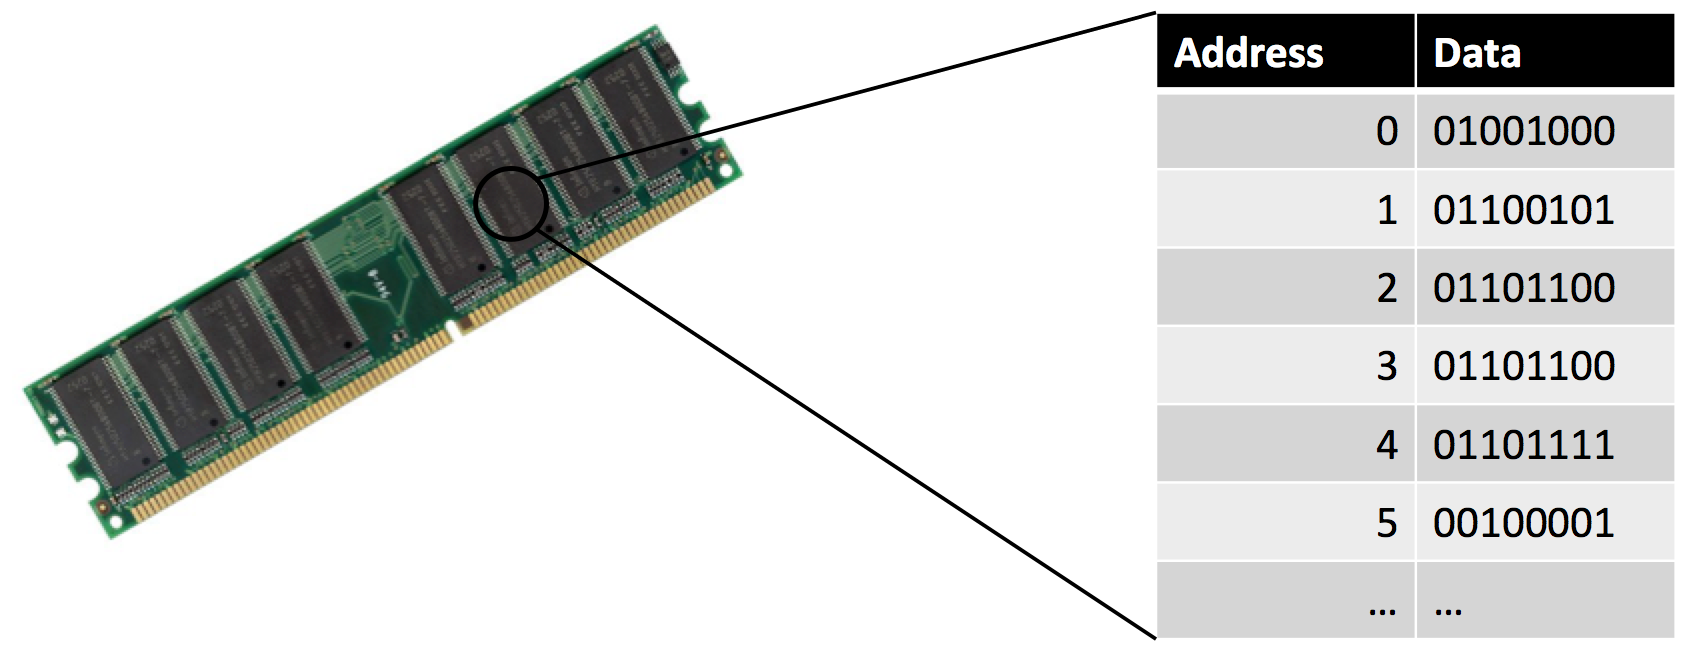
\includegraphics[width=0.8\textwidth]{memory}
	\end{center}
	\begin{itemize}
		\item Memory works like a set of \textbf{boxes}
		\pause\item Each box has a number, its \textbf{address}
		\pause\item Each box contains a \textbf{byte} (8 bits)
	\end{itemize}
\end{frame}

\begin{frame}{Data representation} 
	\begin{itemize}
		\pause\item All data is stored as \textbf{sequences of bytes}
			\begin{itemize}
				\pause\item Sequence of bits, in multiples of 8
				\pause\item Sequence of numbers between 0--255
			\end{itemize}
	\end{itemize}
\end{frame}

\begin{frame}{Integers}
	\begin{itemize}
		\pause\item An \textbf{integer} is a whole number --- positive, negative or zero
		\pause\item Python type: \lstinline{int}
		\pause\item In most languages, \lstinline{int} is limited to 32 or 64 bits
		\pause\item Python uses \textbf{big integers} --- number of bits expands automatically to fit the value to be stored
		\pause\item Stored in memory using binary notation, with 2's complement for negative values
	\end{itemize}
\end{frame}

\begin{frame}{Floating point numbers}
	\begin{itemize}
		\pause\item What about storing non-integer numbers?
		\pause\item Usually we use \textbf{floating point} numbers
		\pause\item Python type: \lstinline{float}
		\pause\item Details on in-memory representation later in the module
		\pause\item (Note: \lstinline{float} in Python 3 has the same precision as \lstinline{double} in C++/C\#/etc)
	\end{itemize}
\end{frame}

\begin{frame}{Integers vs floating point numbers}
	\begin{itemize}
		\pause\item \lstinline{int} and \lstinline{float} are different types!
		\pause\item \lstinline{42} and \lstinline{42.0} are technically different values
			\begin{itemize}
				\pause\item One is an \lstinline{int}, the other is a \lstinline{float}
				\pause\item They are stored differently in memory
				\pause\item However \lstinline{==} etc still know how to compare them sensibly
			\end{itemize}
	\end{itemize}
\end{frame}

\begin{frame}{Booleans}
	\begin{itemize}
		\pause\item A \textbf{boolean} can have one of two values: \textbf{true} or \textbf{false}
		\pause\item Python type: \lstinline{bool}
		\pause\item In Python, we have the keywords \lstinline{True} and \lstinline{False}
		\pause\item Could be represented by a single bit in memory...
		\pause\item ... but since memory is addressed in bytes (or words of multiple bytes),
			usually represented as an \lstinline{int} with $0$ meaning \lstinline{False}
			and any non-zero (e.g.\ $1$) meaning \lstinline{True}
	\end{itemize}
\end{frame}

\begin{frame}[fragile]{Boolean values}
	\begin{itemize}
		\pause\item The \lstinline{if} statement takes a boolean value as its condition:
	\end{itemize}
	\begin{lstlisting}
if x > 10:
    print(x)
	\end{lstlisting}
	\begin{itemize}
		\pause\item Variables can also store boolean values:
	\end{itemize}
	\begin{lstlisting}
result = (x > 10)   # result now stores True or False
if result:
    print(x)
	\end{lstlisting}
\end{frame}

\begin{frame}{The ``None'' value}
	\begin{itemize}
		\pause\item Python has a special value \lstinline{None} which can be used to denote the ``absence'' of any other value
		\pause\item Python type: \lstinline{NoneType}
	\end{itemize}
\end{frame}

\begin{frame}{Strings}
	\begin{itemize}
		\pause\item A \textbf{string} represents a sequence of textual characters
		\pause\item E.g.\ \lstinline{"Hello world!"}
		\pause\item Python type: \lstinline{str}
	\end{itemize}
\end{frame}

\begin{frame}{Strings}
	\begin{itemize}
		\pause\item Stored as sequences of \textbf{characters} encoded as \textbf{integers}
		\pause\item Often \textbf{null-terminated}
			\begin{itemize}
				\pause\item Character number 0 signifies the end of the string
			\end{itemize}
		\pause\item \textbf{ASCII} encodes characters as 8-bit integers
			\begin{itemize}
				\pause\item 255 characters: Latin alphabet, numerals, punctuation
			\end{itemize}
		\pause\item \textbf{UTF-32} encodes characters as 32-bit integers
			\begin{itemize}
				\pause\item \textbf{Unicode} characters: ASCII + several other alphabets, Asian languages, symbols, emoji, ...
			\end{itemize}
		\pause\item \textbf{UTF-8} encodes characters as 8, 16, 24 or 32-bit integers
			\begin{itemize}
				\pause\item More common Unicode characters are smaller $\implies$ more efficient than UTF-32
			\end{itemize}
	\end{itemize}
\end{frame}

{
\setbeamercolor{background canvas}{bg=white}
\begin{frame}[plain]
	\begin{tikzpicture}[remember picture, overlay]
		\node[at=(current page.center)] {
			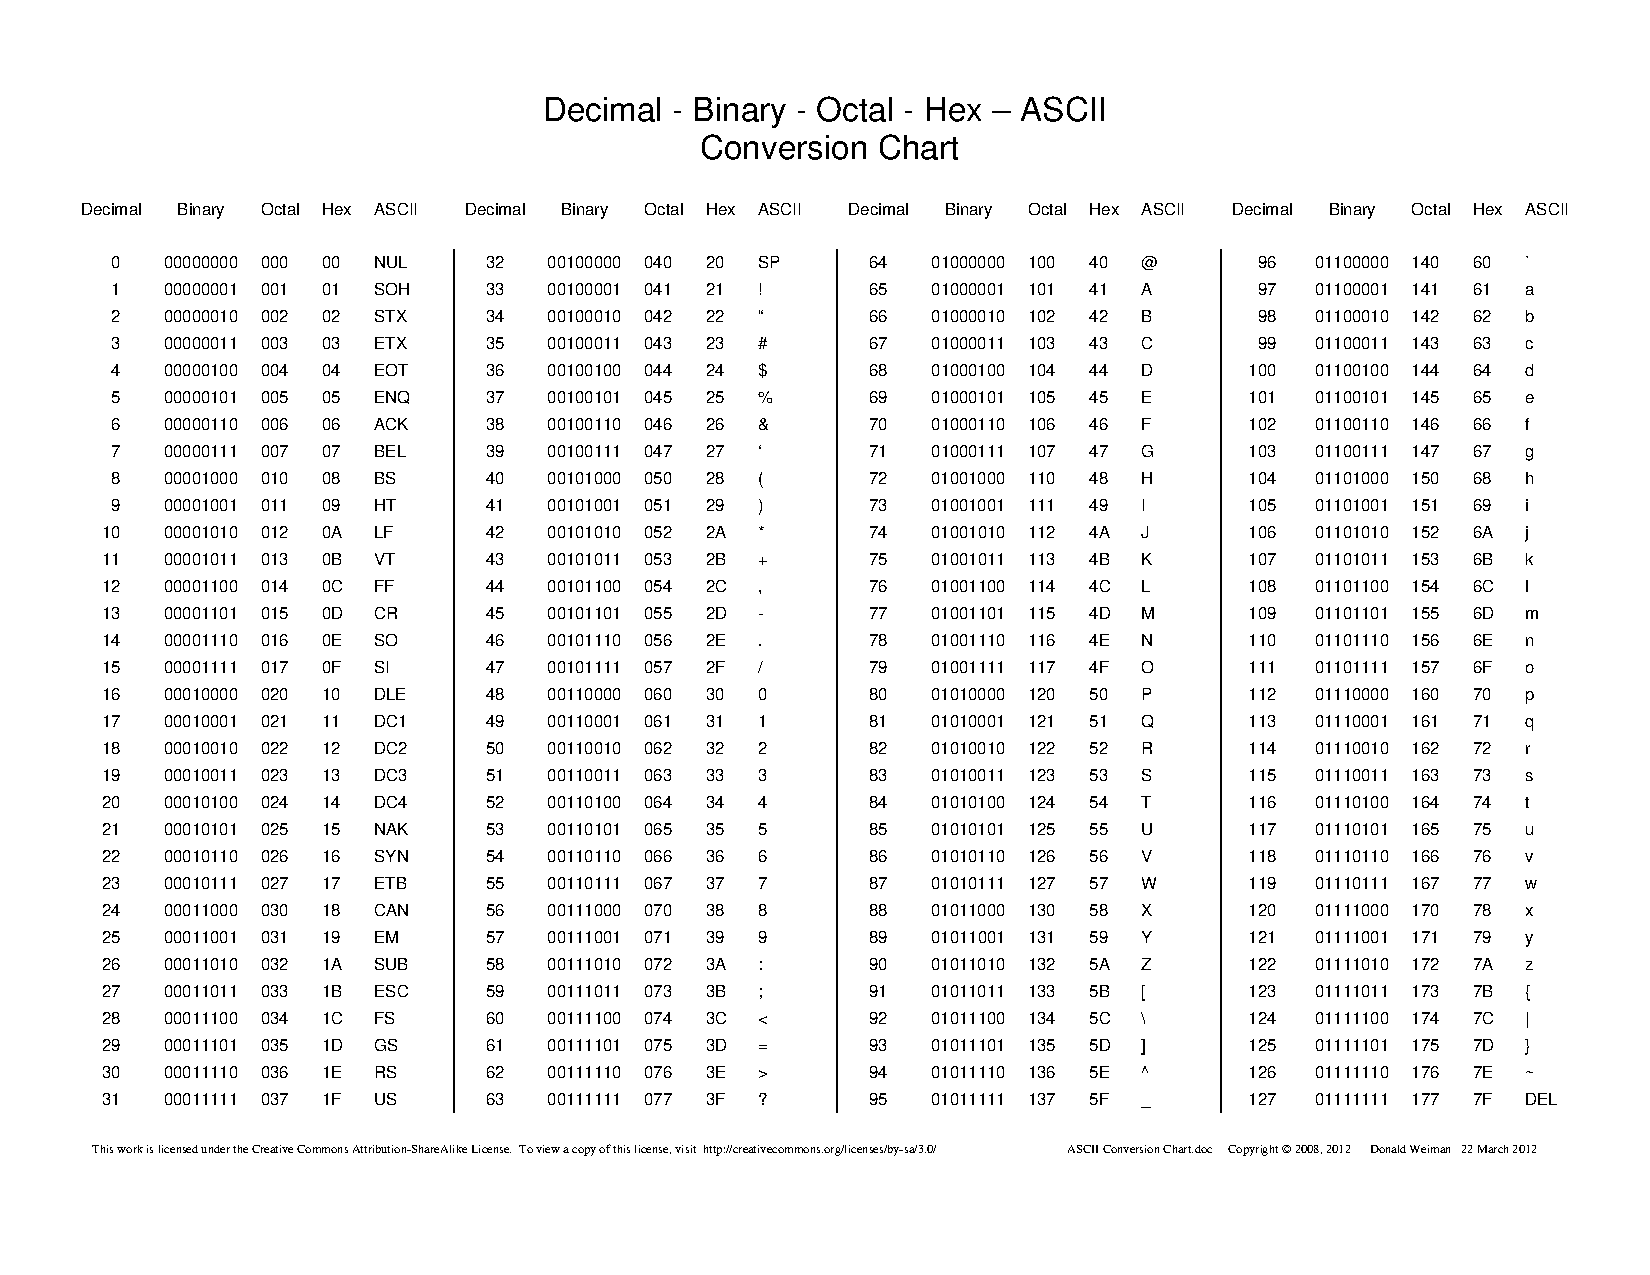
\includegraphics[width=\paperwidth]{ascii_chart}
		};
	\end{tikzpicture}
\end{frame}
}

\begin{frame}{String representation}
	\begin{itemize}
		\pause\item \lstinline{"Hello world!"} in ASCII encoding:
	\end{itemize}
	
	{\footnotesize\pause\begin{tabular}{*{13}{|c}|}
		\hline
		72 & 101 & 108 & 108 & 111 & 32 & 119 & 111 & 114 & 108 & 100 & 33 & 0 \\\hline
	\end{tabular}}
\end{frame}

\begin{frame}{UTF-8 representation}
	\begin{itemize}
		\pause\item For characters in ASCII, UTF-8 is the same:
			\begin{itemize}
				\pause\item a $\to [97]$
			\end{itemize}
		\pause\item Other characters are encoded as multi-byte sequences:
			\begin{itemize}
				\pause\item \"u $\to [195, 188]$
				\pause\item 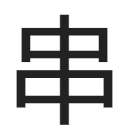
\includegraphics[height=1.5ex]{chinese}\ $\to [228, 184, 178]$
				\pause\item 
\includegraphics[height=1.5ex]{emoji}\ $\to [240, 159, 152, 130]$
			\end{itemize}
	\end{itemize}
\end{frame}

\begin{frame}{Type casting}
	\begin{itemize}
		\pause\item It is often useful to \textbf{cast}, or \textbf{convert}, a value from one type to another
		\pause\item In Python, this is done by calling the type as if it were a function
			\begin{itemize}
				\pause\item \lstinline{float(17)} $\to$ \lstinline{17.0}
				\pause\item \lstinline{int(3.14)} $\to$ \lstinline{3}
				\pause\item \lstinline{str(3.14)} $\to$ \lstinline{"3.14"}
				\pause\item \lstinline{str(1 + 1 == 2)} $\to$ \lstinline{"True"}
				\pause\item \lstinline{int("123")} $\to$ \lstinline{123}
				\pause\item \lstinline{int("five")} gives an error
			\end{itemize}
	\end{itemize}
\end{frame}

\begin{frame}{Other types}
	\begin{itemize}
		\pause\item \textbf{Container} types for collecting several values
			\begin{itemize}
				\pause\item \lstinline{list}, \lstinline{tuple}, \lstinline{dict}, \lstinline{set}, ...
			\end{itemize}
		\pause\item \textbf{Objects}
		\pause\item Almost everything in Python is a value with a type
			\begin{itemize}
				\pause\item Functions, modules, classes, exceptions, ...
				\pause\item Even types themselves are values of type \lstinline{type}!
			\end{itemize}
	\end{itemize}
\end{frame}

